\part{Les notions}
\label{part:theorie}

\chapter{Le problème : louer des machines}

\section{Ce qu'on nous demande}

L'énoncé tient en une phrase : construire une plateforme où un utilisateur
s'inscrit, se connecte, loue une ou plusieurs instances Linux de différentes
distributions pour une durée qu'il choisit, y accède en SSH, et où le service
reste disponible même si une machine du parc tombe.

Derrière cette phrase se cachent dix-sept blocs de travail que le cahier des
charges détaille : l'environnement de développement, l'API web, la base de
données, la conteneurisation, l'infrastructure virtuelle, l'automatisation, un
agent sur chaque nœud, un ordonnanceur, le service de location, le déploiement
des conteneurs, l'accès SSH, l'expiration, la haute disponibilité, la sécurité,
la chaîne d'intégration, les tests, et la documentation.

\begin{notion}{Le vocabulaire du cloud}
Un \textbf{fournisseur de cloud} vend de la capacité de calcul à la demande. On
distingue trois niveaux de service :
\begin{description}
\item[IaaS] \emph{Infrastructure as a Service} --- on vous loue une machine
  nue, vous y installez ce que vous voulez. C'est Amazon EC2, et c'est ce que
  nous construisons.
\item[PaaS] \emph{Platform as a Service} --- on vous loue un endroit où
  déposer votre code, sans vous occuper de la machine. C'est Heroku.
\item[SaaS] \emph{Software as a Service} --- on vous loue un logiciel fini.
  C'est Gmail.
\end{description}
Notre plateforme est donc un mini-IaaS : l'utilisateur reçoit une machine et un
accès root dessus.
\end{notion}

\section{La décision qui structure tout : conteneurs plutôt que VM}

Louer « une machine Linux » peut se faire de deux façons.

\paragraph{Une machine virtuelle.} On émule un ordinateur entier : un noyau
Linux complet, son propre espace mémoire, ses disques virtuels. C'est ce que
fait VirtualBox ou VMware. L'isolation est quasi totale, mais démarrer une VM
prend trente secondes à une minute, et chacune réserve plusieurs centaines de
mégaoctets rien que pour son noyau.

\paragraph{Un conteneur.} On ne démarre pas de second noyau : on réutilise
celui de la machine hôte, en cloisonnant ce que le processus peut voir. Le
démarrage prend moins d'une seconde et le surcoût mémoire est celui des
processus eux-mêmes.

Pour une plateforme qui loue à la minute, la différence est décisive : un
utilisateur n'attend pas une minute après avoir cliqué. Le cahier des charges
tranche d'ailleurs explicitement --- « des conteneurs dans notre cas ».

\begin{figure}[htbp]
\centering
\resizebox{\textwidth}{!}{%
\begin{tikzpicture}[font=\small,
  bloc/.style={draw=grisligne,fill=grisfond,rounded corners=2pt,minimum height=7mm,
               align=center,inner sep=3pt},
  socle/.style={draw=grisligne,fill=white,rounded corners=2pt,minimum height=7mm,align=center}]

\node[font=\small\bfseries] at (2.6,5.1) {Machines virtuelles};
\node[socle,minimum width=5.2cm] at (2.6,0.0) {Matériel};
\node[socle,minimum width=5.2cm] at (2.6,0.8) {Système hôte};
\node[socle,minimum width=5.2cm] at (2.6,1.6) {Hyperviseur};
\foreach \x/\n in {0.95/1, 2.6/2, 4.25/3} {
  \node[bloc,minimum width=1.5cm] at (\x,2.5) {\scriptsize noyau invité};
  \node[bloc,minimum width=1.5cm] at (\x,3.3) {\scriptsize biblioth.};
  \node[bloc,minimum width=1.5cm,fill=bleufond] at (\x,4.1) {\scriptsize appli \n};
}
\draw[decorate,decoration={brace,amplitude=4pt},gristexte]
  (5.45,2.15) -- (5.45,4.45)
  node[midway,right=5pt,gristexte,font=\scriptsize,align=left]
  {chaque VM\\porte son\\propre noyau};

\node[font=\small\bfseries] at (11.2,5.1) {Conteneurs};
\node[socle,minimum width=5.2cm] at (11.2,0.0) {Matériel};
\node[socle,minimum width=5.2cm] at (11.2,0.8) {Système hôte --- \textbf{un seul noyau}};
\node[socle,minimum width=5.2cm] at (11.2,1.6) {Démon Docker};
\foreach \x/\n in {9.55/1, 11.2/2, 12.85/3} {
  \node[bloc,minimum width=1.5cm] at (\x,2.5) {\scriptsize biblioth.};
  \node[bloc,minimum width=1.5cm,fill=bleufond] at (\x,3.3) {\scriptsize appli \n};
}
\draw[decorate,decoration={brace,amplitude=4pt},vertok]
  (14.05,2.15) -- (14.05,3.65)
  node[midway,right=5pt,vertok,font=\scriptsize,align=left]
  {rien entre\\l'appli et le\\noyau de l'hôte};
\end{tikzpicture}}
\caption{La seule vraie différence : le conteneur n'embarque pas de noyau. Tout
le reste --- rapidité de démarrage, consommation mémoire, densité --- en
découle.}
\end{figure}

\begin{piege}{« Un conteneur, c'est une VM légère »}
C'est l'image qu'on donne souvent, et elle induit en erreur. Un conteneur
\emph{partage le noyau de l'hôte}. Conséquences concrètes :
\begin{itemize}
\item on ne peut pas faire tourner un conteneur Windows sur un noyau Linux ;
\item une faille d'évasion du noyau compromet l'hôte \emph{et} tous les autres
  conteneurs --- c'est pourquoi nous retirons les capacités Linux inutiles
  (chapitre~\ref{chap:securite}) ;
\item un conteneur n'a pas de \cmd{init} par défaut : pour y faire tourner
  plusieurs services, il faut en installer un (chapitre~\ref{chap:images}).
\end{itemize}
\end{piege}

\section{Les questions auxquelles il faut répondre}

Dire « on crée un conteneur par location » ne suffit pas. Il faut résoudre ce
que toute plateforme d'hébergement doit résoudre :

\begin{description}
\item[Où placer la machine ?] S'il y a trois serveurs, lequel choisir ? Que
  faire si l'un ne répond plus ?
\item[Comment y accéder ?] Un conteneur n'a pas d'adresse publique. Il faut
  publier un port, et deux machines ne peuvent pas prendre le même.
\item[Comment la faire disparaître ?] Personne ne viendra cliquer sur
  « supprimer » à 3 h du matin. Il faut un service qui surveille les horloges.
\item[Comment garder le secret ?] Le mot de passe root doit être montré à
  l'utilisateur, mais ne doit pas traîner en clair dans une base.
\item[Comment reconstruire tout cela ?] Si le serveur brûle, combien de temps
  faut-il pour remonter la plateforme à l'identique ?
\end{description}

Chacune occupe un chapitre de la partie~\ref{part:construction}.

\chapter{Conteneurs : ce qui se passe réellement}

\section{Trois mécanismes du noyau Linux}

Un conteneur n'est pas un objet du noyau. C'est un processus ordinaire auquel
on a appliqué trois mécanismes.

\begin{notion}{Les espaces de noms (\emph{namespaces})}
Un espace de noms cloisonne \emph{ce qu'un processus peut voir}. Linux en
propose plusieurs, dont :
\begin{description}
\item[PID] le processus se croit seul ; il voit son propre arbre de processus,
  numéroté à partir de 1.
\item[réseau] il a ses propres interfaces, sa table de routage, ses ports. Le
  port 22 du conteneur n'est pas le port 22 de l'hôte.
\item[montage] il a sa propre vision du système de fichiers.
\item[UTS] il a son propre nom de machine.
\end{description}
C'est l'illusion d'être seul au monde.
\end{notion}

\begin{notion}{Les groupes de contrôle (\emph{cgroups})}
Les espaces de noms cloisonnent la \emph{vue} ; les cgroups limitent la
\emph{consommation}. On y plafonne la mémoire, le temps processeur, le nombre
de processus, les entrées-sorties. Sans cgroups, un conteneur parti en boucle
infinie met à genoux tous les autres.

Dans notre projet, ces limites sont posées explicitement à la création :
\cmd{--memory}, \cmd{--memory-reservation}, \cmd{--cpus}, \cmd{--pids-limit}.
\end{notion}

\begin{notion}{Les capacités (\emph{capabilities})}
Historiquement, un processus était soit root (tout permis) soit non-root (rien).
Linux a découpé les pouvoirs de root en une quarantaine de \emph{capacités}
indépendantes : \cmd{CAP\_NET\_BIND\_SERVICE} (écouter sous le port 1024),
\cmd{CAP\_SYS\_ADMIN} (monter des systèmes de fichiers), etc.

On peut donc autoriser un processus à écouter sur le port 22 sans l'autoriser
à charger un module noyau. C'est exactement ce que fait notre durcissement :
retirer tout, puis rendre les dix capacités dont \cmd{sshd} a réellement
besoin.
\end{notion}

\section{Les images et le système de fichiers en couches}

Une \textbf{image} est un modèle figé, en lecture seule. Un \textbf{conteneur}
est une instance en exécution de cette image, avec une fine couche
inscriptible par-dessus.

\begin{figure}[htbp]
\centering
\begin{tikzpicture}[font=\small,
  couche/.style={draw=grisligne,fill=grisfond,minimum width=7.4cm,minimum height=8mm,
                 align=center,inner sep=2pt}]
\node[couche] at (0,0) {\texttt{\scriptsize FROM ubuntu:22.04}\quad\textcolor{gristexte}{\scriptsize 77 Mo}};
\node[couche] at (0,0.85) {\texttt{\scriptsize RUN apt-get install openssh-server ...}\quad\textcolor{gristexte}{\scriptsize 38 Mo}};
\node[couche] at (0,1.7) {\texttt{\scriptsize COPY entrypoint.sh}\quad\textcolor{gristexte}{\scriptsize 4 Ko}};
\node[couche,fill=bleufond,draw=bleutrait] at (0,2.75)
  {\scriptsize couche inscriptible du conteneur\quad\textcolor{bleutrait}{\scriptsize vide au départ}};
\draw[decorate,decoration={brace,amplitude=5pt},gristexte]
  (3.9,-0.42) -- (3.9,2.12)
  node[midway,right=6pt,gristexte,font=\scriptsize,align=left]
  {l'\textbf{image} :\\en lecture seule,\\partagée entre tous\\les conteneurs};
\draw[decorate,decoration={brace,amplitude=5pt},bleutrait]
  (3.9,2.35) -- (3.9,3.15)
  node[midway,right=6pt,bleutrait,font=\scriptsize,align=left]
  {le \textbf{conteneur} :\\jetable};
\end{tikzpicture}
\caption{Une image est un empilement de couches. Dix conteneurs issus de la
même image ne stockent la base qu'une fois : seule la couche du dessus leur est
propre.}
\end{figure}

Cette architecture a une conséquence qu'on oublie vite : \textbf{détruire un
conteneur détruit sa couche inscriptible}, donc tout ce que l'utilisateur y a
écrit. C'est pourquoi le projet sauvegarde le travail avant destruction
(chapitre~\ref{chap:archives}) et pourquoi la reprise après panne ne rend pas
les fichiers (chapitre~\ref{chap:ha}).

\begin{retenir}
Une image, c'est la recette figée. Un conteneur, c'est le plat : on le mange,
on jette l'assiette. Tout ce qui doit survivre est rangé ailleurs --- dans un
volume, dans une base, ou dans une archive.
\end{retenir}

\section{Les commandes qu'il faut connaître}

\begin{lstlisting}[language=bash]
# Construire une image a partir du Dockerfile du dossier courant
docker build -t mon_image:latest .

# Lancer un conteneur en arriere-plan (-d), en publiant un port
docker run -d --name ma_machine -p 2222:22 mon_image:latest

# Lister ce qui tourne ; -a ajoute ce qui est arrete
docker ps
docker ps -a --filter "label=insacloud.role=rented-machine"

# Entrer dans un conteneur qui tourne
docker exec -it ma_machine /bin/bash

# Comprendre pourquoi il ne demarre pas
docker logs ma_machine

# Tout savoir de sa configuration reelle (ports, limites, capacites)
docker inspect ma_machine

# Le detruire, meme s'il tourne
docker rm -f ma_machine
\end{lstlisting}

\begin{notion}{Publier un port}
\cmd{-p 2222:22} signifie : « ce qui arrive sur le port \textbf{2222 de
l'hôte} est transmis au port \textbf{22 du conteneur} ». Le conteneur croit
écouter sur 22 ; le monde extérieur frappe sur 2222.

C'est le mécanisme qui permet de faire tourner cent serveurs SSH sur une seule
machine : chacun écoute son 22 interne, mais reçoit un port externe différent.
Notre plateforme en attribue un dans la plage 8000--9000 et garantit l'unicité
par un index en base (chapitre~\ref{chap:bdd}).
\end{notion}

\chapter{Une application web, de bout en bout}

\section{Ce qui se passe quand on tape une adresse}

\begin{figure}[htbp]
\centering
\resizebox{\textwidth}{!}{%
\begin{tikzpicture}[font=\scriptsize,
  b/.style={draw=grisligne,fill=grisfond,rounded corners=2pt,minimum height=12mm,
            minimum width=2.1cm,align=center},
  f/.style={-{Stealth[length=2mm]},gristexte}]
\node[b] (nav) at (0,0) {Navigateur\\\textcolor{gristexte}{Firefox}};
\node[b] (ngx) at (3,0) {nginx\\\textcolor{gristexte}{port 443}};
\node[b] (gun) at (6,0) {Gunicorn\\\textcolor{gristexte}{port 5000}};
\node[b] (fl) at (9,0) {Flask\\\textcolor{gristexte}{votre code}};
\node[b] (db) at (12,0) {PostgreSQL\\\textcolor{gristexte}{port 5432}};
\draw[f] (nav) -- node[above]{HTTPS} (ngx);
\draw[f] (ngx) -- node[above]{HTTP} node[below]{local} (gun);
\draw[f] (gun) -- node[above]{WSGI} (fl);
\draw[f] (fl) -- node[above]{SQL} (db);
\draw[{Stealth[length=2mm]}-,gristexte,dashed] (nav.south) ++(0,-0.5)
  -- ++(12,0) node[midway,below,gristexte]{la réponse repart par le même chemin};
\draw[gristexte,dashed] (db.south) -- ++(0,-0.5);
\end{tikzpicture}}
\caption{La chaîne complète d'une requête. Chaque maillon a une raison d'être
précise.}
\end{figure}

\paragraph{Pourquoi nginx devant ?} Flask sait répondre à du HTTP, mais n'est
pas prévu pour affronter Internet. On place donc un \emph{proxy inverse}
devant : nginx termine le TLS (le « s » de HTTPS), sert les fichiers statiques
--- images, CSS --- sans réveiller Python, impose des en-têtes de sécurité, et
protège l'application des requêtes malformées.

\begin{notion}{Proxy direct et proxy inverse}
Un \textbf{proxy direct} agit pour le client : votre navigateur passe par lui
pour atteindre le web. Un \textbf{proxy inverse} agit pour le serveur : le
client croit parler au site, alors qu'il parle à nginx, qui relaie. Le premier
cache qui demande, le second cache qui répond.
\end{notion}

\paragraph{Pourquoi Gunicorn ?} Le serveur de développement de Flask traite une
requête à la fois et le dit lui-même : « ne pas utiliser en production ».
Gunicorn lance plusieurs processus ouvriers qui se partagent les requêtes,
redémarre ceux qui plantent, et sait s'arrêter proprement.

\begin{notion}{WSGI}
\emph{Web Server Gateway Interface} est le contrat entre un serveur Python et
une application Python. L'application expose un objet appelable qui reçoit un
dictionnaire décrivant la requête et renvoie une réponse. Grâce à ce contrat,
on remplace Gunicorn par uWSGI ou Waitress sans toucher une ligne de Flask.
\end{notion}

\begin{piege}{Un seul processus Gunicorn n'est pas une option}
Avec un seul ouvrier, une requête lente --- créer un conteneur prend plusieurs
secondes --- bloque \emph{tous} les autres utilisateurs. Notre déploiement en
lance quatre. Mais plusieurs processus qui démarrent simultanément posent un
autre problème, celui de la course à l'initialisation de la base : nous y
revenons au chapitre~\ref{chap:bdd}, car il nous a réellement coûté une panne.
\end{piege}

\section{Flask en dix minutes}

Flask est un \emph{micro}-framework : il fournit le routage, les gabarits et
les sessions, et laisse le reste à des bibliothèques que vous choisissez. C'est
l'inverse de Django, qui décide à votre place.

\begin{lstlisting}[language=Python]
from flask import Flask, render_template, request, redirect, url_for, session

app = Flask(__name__)
app.secret_key = "..."           # sert a SIGNER les cookies de session

@app.route("/")                  # une URL ...
def accueil():                   # ... associee a une fonction
    return render_template("index.html", titre="Bonjour")

@app.route("/login", methods=["GET", "POST"])
def login():
    if request.method == "POST":
        session["user"] = request.form["username"]   # cookie signe
        return redirect(url_for("accueil"))
    return render_template("login.html")
\end{lstlisting}

\begin{description}
\item[Le routage] \cmd{@app.route} associe un chemin d'URL à une fonction. La
  fonction renvoie ce que le navigateur recevra.
\item[Les gabarits] \cmd{render\_template} remplit un fichier HTML avec des
  variables, grâce au moteur Jinja2.
\item[La session] \cmd{session} est un dictionnaire stocké \emph{dans un
  cookie} chez le client.
\end{description}

\begin{piege}{Une session Flask est signée, pas chiffrée}
C'est l'erreur la plus courante, et nous l'avons commise. Le contenu d'un
cookie de session est encodé en base64 : \textbf{n'importe qui peut le lire},
sans la clé. La signature empêche seulement de le \emph{modifier}.

Nous y avions mis le mot de passe root d'une machine, le temps de l'afficher
une fois. Il suffisait d'ouvrir les outils du navigateur pour le récupérer. La
correction consiste à ne stocker que l'identifiant de la machine et à relire le
secret en base, chiffré (chapitre~\ref{chap:securite}).
\end{piege}

\section{Le même chemin pour un humain et pour un programme}

Un trait d'architecture qui revient partout dans ce projet : chaque route sert
soit du HTML, soit du JSON, selon ce que l'appelant demande dans l'en-tête
\cmd{Accept}. Il n'y a donc pas un site d'un côté et une API de l'autre, mais
une seule logique métier avec deux rendus.

\begin{lstlisting}[language=Python,caption={\fichier{2\_webapp/app.py} --- choisir le format de la réponse}]
def veut_json() -> bool:
    # Un client qui accepte TOUT (Accept: */*, cas de curl sans en-tete)
    # n'est pas un client d'API : seul celui qui demande du JSON sans accepter
    # le HTML est traite comme tel.
    accepte = request.accept_mimetypes
    return accepte.accept_json and not accepte.accept_html
\end{lstlisting}

\begin{piege}{\texttt{Accept: */*} n'est pas une demande de JSON}
Notre première version répondait du JSON à tout client acceptant
\cmd{application/json} --- ce que fait \cmd{*/*}. Résultat : certains
navigateurs et tous les \cmd{curl} nus recevaient du JSON à la place de la
page. La condition correcte est : \emph{accepte le JSON} \textbf{et}
\emph{n'accepte pas le HTML}.
\end{piege}

\chapter{L'infrastructure décrite dans des fichiers}

\section{Le problème du « ça marche chez moi »}

Un projet installé à la main sur un serveur a une propriété désastreuse :
personne, pas même son auteur, ne sait exactement ce qui a été fait. Au
remontage, il manque toujours un paquet, un fichier de configuration, une
permission.

L'\emph{infrastructure as code} consiste à écrire l'état voulu dans des
fichiers versionnés, et à laisser un outil l'appliquer. Deux outils se
partagent le travail.

\begin{description}
\item[Vagrant] crée les machines virtuelles : combien, à partir de quelle
  image, avec quelle mémoire, quelle adresse.
\item[Ansible] les configure : installe les paquets, dépose les fichiers,
  démarre les services.
\end{description}

\section{Vagrant : des VM reproductibles}

\begin{lstlisting}[language=Ruby,caption={Le principe, en quelques lignes}]
Vagrant.configure("2") do |config|
  config.vm.box = "bento/ubuntu-22.04"       # l'image de base
  config.vm.define "worker1" do |node|
    node.vm.hostname = "worker1"
    node.vm.network "private_network", ip: "192.168.56.11"
    node.vm.provider "virtualbox" do |v|
      v.memory = 3072
      v.cpus   = 2
    end
  end
end
\end{lstlisting}

\cmd{vagrant up} lit ce fichier et crée la VM ; \cmd{vagrant destroy} l'efface.
Entre les deux, l'état est entièrement décrit par le fichier : n'importe qui,
sur n'importe quelle machine, obtient le même résultat.

\begin{notion}{\emph{Box} et \emph{provider}}
Une \textbf{box} est une image de VM préfabriquée, téléchargée depuis un
catalogue public. Un \textbf{provider} est le logiciel de virtualisation qui
l'exécute : VirtualBox, VMware, Parallels, QEMU. Le même \cmd{Vagrantfile} peut
cibler plusieurs providers --- indispensable ici, car VirtualBox ne fonctionne
pas sur les Mac à puce Apple.
\end{notion}

\section{Ansible : décrire l'état, pas les étapes}

Ansible se connecte en SSH et applique des \emph{tâches}. La différence avec un
script shell est fondamentale.

\begin{lstlisting}[language=bash,caption={Un script shell décrit des actions}]
apt-get install -y nginx          # se comporte mal si deja installe
mkdir /etc/insacloud              # echoue si le dossier existe
echo "..." > /etc/insacloud/conf  # ecrase a chaque fois
systemctl restart nginx           # redemarre meme si rien n'a change
\end{lstlisting}

\begin{lstlisting}[language=yamlplus,caption={Ansible décrit un état voulu}]
- name: nginx est installe
  ansible.builtin.apt:
    name: nginx
    state: present

- name: Le dossier de configuration existe, avec les bons droits
  ansible.builtin.file:
    path: /etc/insacloud
    state: directory
    owner: insacloud
    mode: "0750"

- name: La configuration est en place
  ansible.builtin.template:
    src: insacloud.conf.j2
    dest: /etc/insacloud/conf
  notify: Redemarrer nginx        # UNIQUEMENT si le fichier a change
\end{lstlisting}

\begin{notion}{Idempotence}
Une opération est \textbf{idempotente} si l'appliquer deux fois donne le même
résultat que l'appliquer une fois. C'est la propriété centrale d'Ansible :
relancer le playbook sur un serveur déjà configuré ne doit \emph{rien} changer.

La preuve se lit dans le compte rendu : au second passage, \cmd{changed=0}.
Dans ce projet, c'est mesuré sur les quatre nœuds à chaque modification
(chapitre~\ref{chap:ansible}).
\end{notion}

\begin{retenir}
Idempotent ne veut pas dire « ne fait rien la deuxième fois », mais « vérifie
l'état, et n'agit que s'il diffère de celui qui est voulu ». La nuance compte :
c'est elle qui permet de relancer le déploiement sans crainte, à n'importe quel
moment.
\end{retenir}

\paragraph{Le vocabulaire d'Ansible.}
\begin{description}
\item[Inventaire] la liste des machines, rangées par groupes
  (\cmd{[controllers]}, \cmd{[workers]}).
\item[Tâche] une action unitaire, exprimée par un \emph{module} :
  \cmd{apt}, \cmd{file}, \cmd{template}, \cmd{systemd}.
\item[Rôle] un ensemble de tâches réutilisable, avec ses variables par défaut,
  ses fichiers et ses gabarits. Le projet en compte neuf.
\item[Playbook] la partition : quels rôles sur quels groupes, dans quel ordre.
\item[Handler] une tâche qui ne s'exécute que si une autre a changé quelque
  chose. Typiquement : redémarrer un service.
\item[Vault] un fichier chiffré où ranger les secrets, versionnable sans
  danger.
\end{description}

\chapter{DevSecOps : pourquoi une chaîne automatique}

\section{Le constat}

Un projet d'école finit souvent par ne plus fonctionner que sur la machine de
son auteur, parce que rien ne vérifie le contraire. L'intégration continue
consiste à faire tourner, à chaque envoi de code, l'ensemble des contrôles que
personne n'a le courage de relancer à la main.

Le « Sec » de DevSecOps signifie que la sécurité fait partie de ces contrôles
automatiques, plutôt que d'être un audit ponctuel en fin de projet.

\section{Les familles de contrôles}

\begin{description}
\item[Lint] lit le code sans l'exécuter et signale ce qui est douteux :
  variable jamais utilisée, import mort, nom inconnu. Outils : \cmd{ruff} pour
  Python, \cmd{hadolint} pour les Dockerfiles, \cmd{ansible-lint}.
\item[Tests] exécutent le code sur des cas connus et comparent au résultat
  attendu. Outil : \cmd{pytest}.
\item[SAST] \emph{Static Application Security Testing} --- cherche des motifs
  dangereux dans le source : concaténation SQL, secret en dur, appel système
  construit à partir d'une entrée utilisateur. Outil : \cmd{bandit}.
\item[SCA] \emph{Software Composition Analysis} --- confronte la liste des
  dépendances aux bases de vulnérabilités publiques. Outil : \cmd{pip-audit}.
\item[Recherche de secrets] cherche clés et mots de passe commis par erreur,
  \emph{y compris dans l'historique} : effacer un secret dans un commit
  ultérieur ne l'efface pas du dépôt. Outil : \cmd{gitleaks}.
\item[DAST] \emph{Dynamic Application Security Testing} --- attaque
  l'application \emph{en fonctionnement} : en-têtes manquants, pages
  accessibles sans authentification, jetons CSRF absents. Outils : un script
  maison et \cmd{nuclei}.
\item[Scan d'image] cherche les CVE des paquets du système de base de l'image.
  Outil : \cmd{Trivy}.
\item[SBOM] \emph{Software Bill of Materials} --- l'inventaire exhaustif de ce
  qui est livré, conservé pour pouvoir répondre plus tard à « sommes-nous
  touchés par telle faille ? ». Outil : \cmd{Syft}.
\end{description}

\begin{figure}[htbp]
\centering
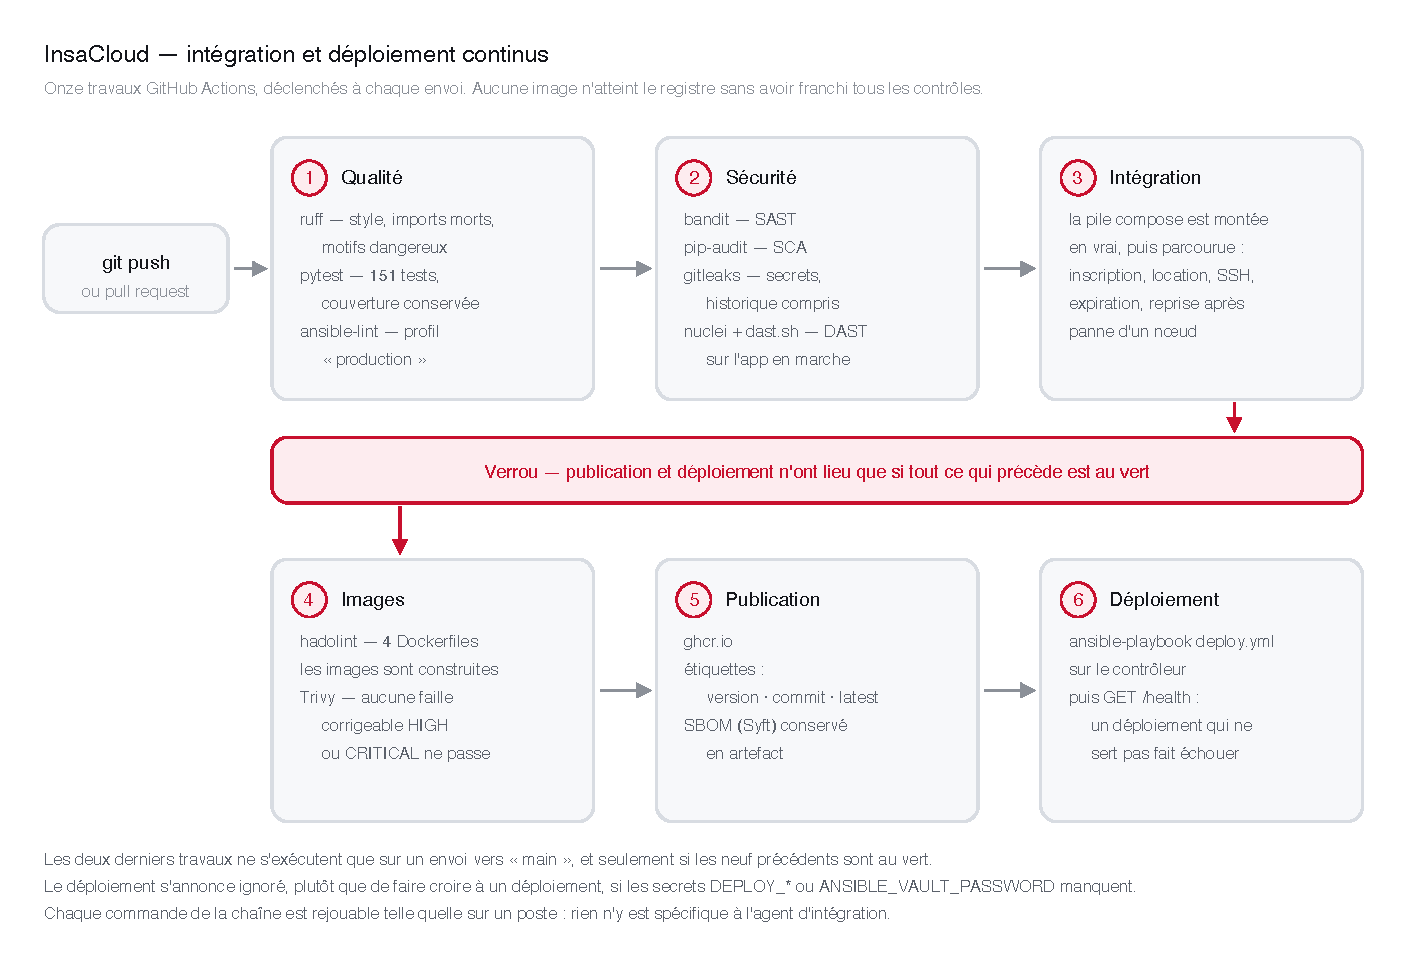
\includegraphics[width=\textwidth]{figures/chaine-ci-cd.pdf}
\caption{La chaîne réelle du projet : onze travaux, détaillés au
chapitre~\ref{chap:ci}.}
\end{figure}

\begin{notion}{CVE}
\emph{Common Vulnerabilities and Exposures} --- l'identifiant mondial unique
d'une faille connue, de la forme \cmd{CVE-2024-12345}. Les outils de SCA et de
scan d'image travaillent tous avec ces identifiants.
\end{notion}

\begin{retenir}
Une chaîne d'intégration n'est utile que si elle \emph{bloque}. Un contrôle qui
affiche un avertissement que personne ne lit ne sert à rien. Ici, aucune image
n'atteint le registre si l'un des contrôles échoue --- et c'est arrivé : nos
propres images ont été refusées par notre propre scan
(chapitre~\ref{chap:ci}).
\end{retenir}
